\documentclass[11pt]{article}

\usepackage[margin=0.70in]{geometry}
\usepackage{amssymb}
\usepackage{booktabs}
\usepackage{caption}
\usepackage[american]{circuitikz}
\usepackage{enumitem}
\usepackage{fancyhdr}
\usepackage{graphicx}
\usepackage[table]{xcolor}
\usepackage[hidelinks]{hyperref}
\usepackage{listings}
\usepackage{microtype}
\usepackage{tabularx}
\usepackage{tikz}
\usepackage{titlesec}
\graphicspath{{docs/lessons/assets/}{../assets/}}

\definecolor{AdkBlue}{gray}{0.125}
\definecolor{AdkRed}{gray}{0}
\definecolor{AdkGreen}{gray}{0.315}
\definecolor{CodeGray}{gray}{0.969}

\hypersetup
{
    pdftitle={ADK Lesson 005: Passive Piezo Sounder},
    pdfauthor={Kevin Shanahan},
    pdfsubject={Timer ownership, explicit time, deterministic tone tests, and safe Mega 2560 wiring},
    pdflang={en-US}
}
\pagestyle{fancy}
\fancyhf{}
\lhead{\textsc{ADK Lesson 005}}
\rhead{Passive piezo sounder}
\cfoot{\thepage}
\setlength{\headheight}{14pt}
\setlength{\parindent}{0pt}
\setlength{\parskip}{5pt}
\setlist{nosep,leftmargin=1.45em}
\titleformat{\section}{\Large\bfseries\color{AdkBlue}}{\thesection}{0.5em}{}
\titleformat{\subsection}{\large\bfseries\color{AdkBlue}}{\thesubsection}{0.5em}{}

\lstdefinestyle{adkcpp}
{
    language=C++,
    backgroundcolor=\color{CodeGray},
    basicstyle=\ttfamily\small,
    keywordstyle=\color{AdkBlue}\bfseries,
    commentstyle=\color{AdkGreen},
    columns=fullflexible,
    keepspaces=true,
    showstringspaces=false,
    frame=single,
    rulecolor=\color{black!20},
    breaklines=true,
    tabsize=4
}

\newcommand{\checkbox}{\(\square\)}
\newcommand{\blank}[1]{\rule{#1}{0.4pt}}
\newcommand{\warningbox}[1]{%
    \begin{center}
    \fcolorbox{AdkRed}{AdkRed!6}{\parbox{0.91\linewidth}
    {\textbf{\color{AdkRed}Safety checkpoint.} #1}}
    \end{center}}
\newcommand{\evidencebox}[1]{%
    \begin{center}
    \fcolorbox{AdkBlue}{AdkBlue!5}{\parbox{0.91\linewidth}{#1}}
    \end{center}}

\begin{document}

\begin{center}
    {\Huge\bfseries Passive Piezo Sounder}\\[4pt]
    {\Large Audible cues without blocking the loop}\\[8pt]
    \textit{Own the timer, pass time explicitly, and make silence the safe state.}
\end{center}

\begin{tabularx}{\linewidth}{@{}>{\bfseries}l X >{\bfseries}l X@{}}
Lesson & 005 --- component & Time & 80--110 minutes\\
Requires & Digital output and explicit time & Board & Arduino Mega 2560\\
Output & Passive piezo on D6 & Status & host verified; hardware experimental\\
Safety & E1: identified logic-level passive piezo only & Power & Mega USB only\\
\end{tabularx}

\section{Why sound is a resource problem}

A tone looks like a simple output, but it couples a pin to a hardware timer.
ADK's \texttt{PiezoSounder} claims both resources before it touches the circuit.
If either is busy, initialization fails predictably. Once initialized,
\texttt{play()} starts a square wave and returns immediately. The main loop remains
free to scan buttons, update LEDs, and enforce deadlines.

\subsection*{Learning targets}

By the end, you can:

\begin{itemize}
    \item distinguish a passive piezo transducer from an active buzzer or speaker;
    \item wire a modest passive piezo load to Mega D6 with a series resistor;
    \item explain why tone owns D6 and Timer2;
    \item schedule and stop a tone using explicit \texttt{TimePoint} values;
    \item predict pin and timer claim conflicts before hardware changes;
    \item verify duration, replacement, shutdown, and rollover deterministically;
    \item show that stop, shutdown, and destruction return the endpoint to silence.
\end{itemize}

\section{Part boundary and safety}

\warningbox{Use only a small \emph{passive piezo transducer} documented for
logic-level excitation. Do not substitute an 8\,$\Omega$ speaker, magnetic
sounder, siren, active buzzer module, amplifier, or unknown part. Disconnect USB
and every other power source before changing wiring. Begin with short tones at a
comfortable distance; stop if sound is painful, startling, or causes discomfort.}

\textbf{Identify the part before building:}

\begin{itemize}
    \item A passive piezo needs an alternating waveform; steady DC produces at
          most a click. Kits may label it ``passive buzzer''.
    \item An active buzzer contains an oscillator and sounds from steady DC. It is
          a different component and is not used here.
    \item A dynamic speaker is a low-impedance inductive load. A Mega pin must not
          drive it directly.
\end{itemize}

\evidencebox{\textbf{Transistor/speaker boundary.} A speaker, high-current
sounder, or louder transducer requires a separately designed driver: a suitable
transistor or amplifier, current limiting, supply analysis, common-ground or
isolation decision, and inductive protection where the load requires it. That
driver is outside this lesson. A transistor is not permission to guess a load's
ratings.}

\textbf{Required:} Mega 2560, USB data cable, breadboard, one passive piezo
transducer, one 100\,$\Omega$ series resistor, and jumper wires. Use the
transducer datasheet when its permitted voltage or wiring differs.
Record the manufacturer's part number, rated voltage, and capacitance or drive
limits before energizing it. If the kit part cannot be identified well enough
to establish those limits, keep the exercise host-only.

\section{Predict before wiring}

\begin{center}
\begin{tabularx}{\linewidth}{@{}p{0.25\linewidth}p{0.28\linewidth}X@{}}
\toprule
Action & Expected software state & Expected circuit state\\
\midrule
Construct only & not initialized, not sounding & D6 untouched\\
Initialize & initialized, not sounding & D6 passive; Timer2 owned\\
Play 440\,Hz for 250\,ms & sounding at 440\,Hz & square wave drives piezo\\
Update before deadline & still sounding & waveform continues\\
Update at/after deadline & not sounding & tone stopped; D6 restored to input\\
Shutdown or destruction & not initialized, not sounding & silence; claims released\\
\bottomrule
\end{tabularx}
\end{center}

\textbf{Conflict prediction:} If another component owns Timer2, which status
should \texttt{initialize()} return? \blank{1.5in}\\
Should D6 change mode? \blank{0.8in}\quad Why?\\[8pt]
\blank{6.8in}

\section{Exact Mega 2560 circuit}

\begin{figure}[ht]
    \centering
    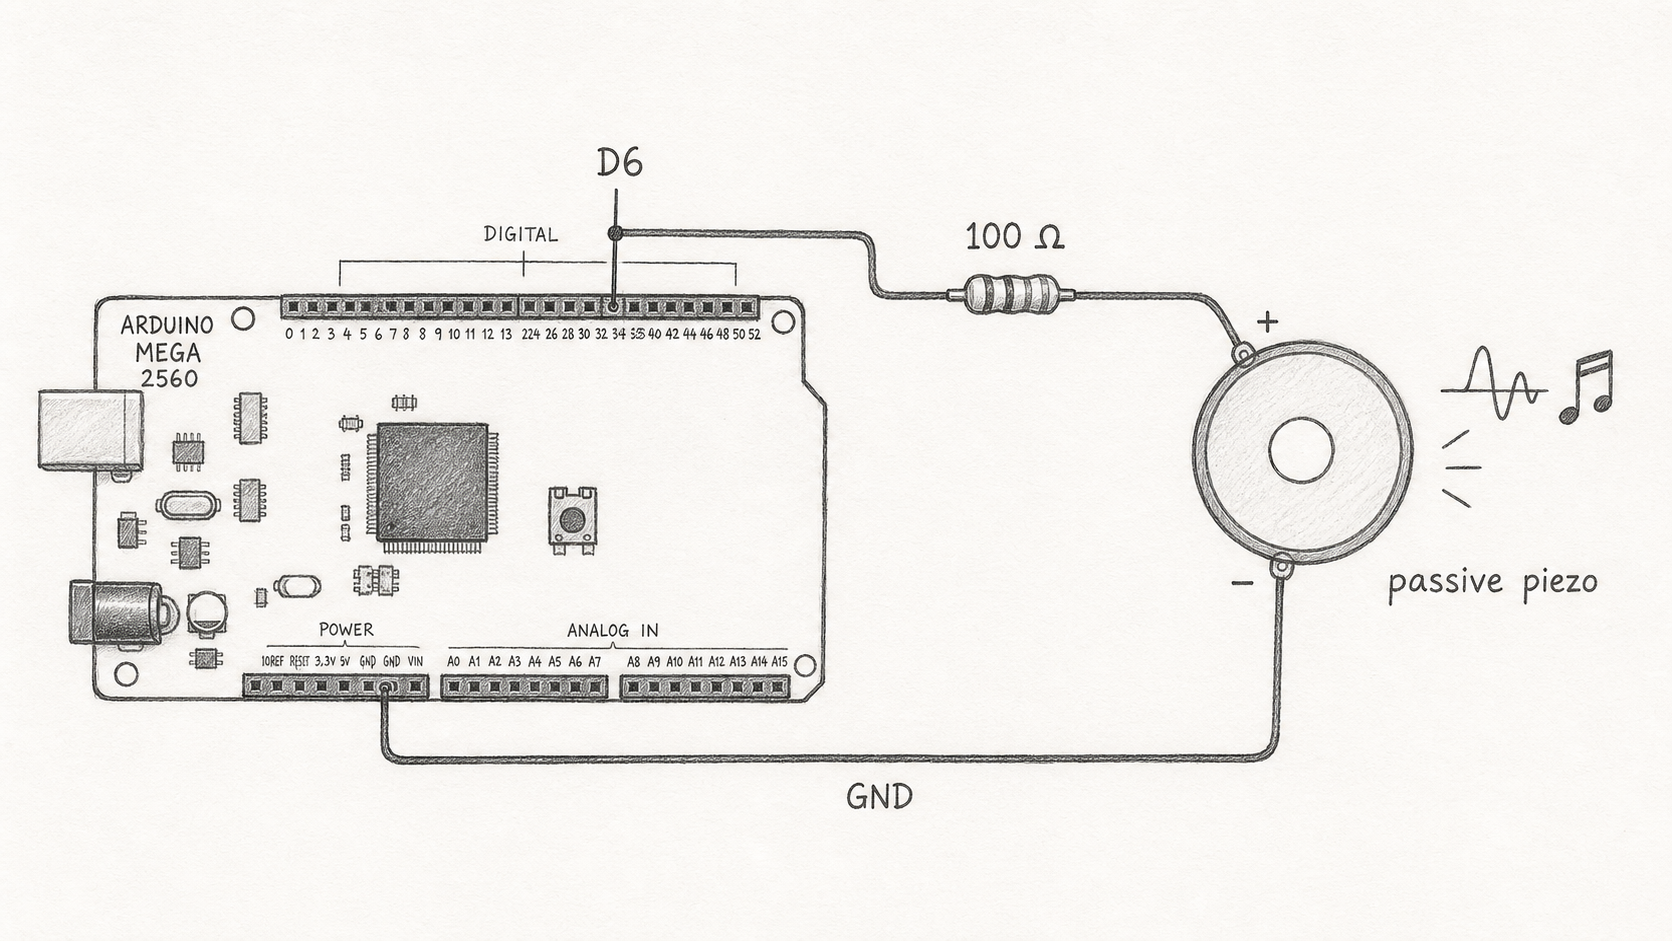
\includegraphics[width=\linewidth,height=0.30\textheight,keepaspectratio]
        {005-piezo-pencil.png}
    \caption*{\textbf{Orientation only.} This drawing identifies the intended
    parts and signal path, but pin spacing and board geometry are illustrative.
    The exact schematic and connection table below are authoritative. Trace D6,
    100\,$\Omega$, passive piezo, and Mega GND before applying power.}
\end{figure}

\begin{center}
\begin{circuitikz}
    \draw
        (0,2.2) node[left]{Mega D6}
        to[short,o-] (0.8,2.2)
        to[R,l={100\,$\Omega$}] (3.2,2.2)
        to[piezoelectric,l={passive piezo}] (5.7,2.2)
        -- (5.7,0.4) node[ground]{};
    \node[align=left,anchor=west] at (6.6,1.8)
        {Use one Mega GND pin.\\
         If the piezo is marked \(+\),\\
         place \(+\) toward D6.};
\end{circuitikz}
\end{center}

\begin{center}
\begin{tabular}{@{}lll@{}}
\toprule
From & Through & To\\
\midrule
Mega D6 & 100\,$\Omega$ resistor & passive piezo signal / \(+\) terminal\\
piezo return / \(-\) terminal & jumper & Mega GND\\
\bottomrule
\end{tabular}
\end{center}

The resistor limits edge current into the piezo's capacitance and makes the
exercise conservative; it does not make an arbitrary load safe. Do not connect a
separate 5\,V wire. Keep leads short. With power disconnected, verify no
continuity from 5\,V to GND and trace D6 through the resistor and piezo to GND.

\section{Use the exact interface}

\begin{lstlisting}[style=adkcpp]
#include <Adk.h>

constexpr adk::PinId                   SounderPin = 6;
constexpr adk::PiezoSounder::Frequency CueHz      = 440;
const adk::Duration                    CueLength  (250);

adk::Runtime      runtime;
adk::PiezoSounder sounder (runtime.resources (), SounderPin);

void setup ()
{
    const adk::Status status = sounder.initialize ();

    if (!status.ok ())
    {
        return;
    }

    const adk::TimePoint now (millis ());
    sounder.play (CueHz, CueLength, now);
}

void loop ()
{
    const adk::TimePoint now (millis ());
    sounder.update (now);
}
\end{lstlisting}

\texttt{play(frequency, duration, now)} accepts 31--20,000\,Hz and a duration of
1--60,000\,ms. Zero duration, an out-of-range frequency, or an excessive duration
returns a status whose
\texttt{error() == StatusCode::InvalidArgument} without starting a new tone.
\texttt{play()} before initialization reports
\texttt{error() == StatusCode::NotInitialized}.

The API does not call \texttt{delay()}. It stores the supplied start time and
duration. Each \texttt{update(now)} compares the caller's time with the deadline.
The caller therefore controls replay, test time, and loop cadence.

\subsection{Lifecycle and replacement}

Construction only stores the registry and pin. Successful initialization claims
D6 first, then Timer2. If Timer2 is unavailable, the D6 claim is rolled back.
Repeated successful initialization is harmless.

A successful \texttt{play()} while already sounding replaces the frequency,
duration, and start time. It does not queue a tone. \texttt{stop()} is idempotent:
it calls the platform stop operation only while sounding, clears the audible
state, and returns D6 to input mode. \texttt{shutdown()} stops first, releases
Timer2 and D6, and is also idempotent. The destructor calls shutdown, so cleanup
remains correct in an exception-using host environment even though ADK throws no
exceptions internally.

\section{Timer2 ownership}

On the Mega 2560 target, this implementation models Arduino tone generation as
exclusive ownership of timer index 2. Timer2 is also associated with hardware PWM
channels on Mega pins 9 and 10. Board-aware PWM code and PiezoSounder must therefore
agree through the same \texttt{ResourceRegistry}; incompatible use fails instead
of silently changing frequency or breaking a tone.

\begin{center}
\begin{tabularx}{\linewidth}{@{}p{0.25\linewidth}p{0.24\linewidth}X@{}}
\toprule
Existing owner & Sounder initialization & Required evidence\\
\midrule
D6 pin owner & \texttt{error(): ResourceBusy} & no pin mode or tone call\\
Timer2 owner & \texttt{error(): ResourceBusy} & D6 claim rolled back; no hardware call\\
Unrelated pin/timer owner & \texttt{ok(): true} & D6 and Timer2 claimed\\
Same initialized sounder & \texttt{ok(): true} & no repeated hardware work\\
\bottomrule
\end{tabularx}
\end{center}

\warningbox{A registry can prevent conflicts only when every participating
component uses that registry and the board map describes the shared timer
correctly. Direct calls to Arduino \texttt{tone()}, \texttt{analogWrite()}, or
third-party timer libraries bypass ADK ownership. Do not mix them in this lesson.}

\section{Deterministic host tests}

The implementation is host verified with fake Arduino tone operations. Add or
review tests that drive exact time values; never sleep in a correctness test.

\begin{lstlisting}[style=adkcpp]
fake::reset ();
adk::ResourceRegistry resources;
adk::PiezoSounder     sounder (resources, 6);

require (sounder.initialize ().ok ());
require (sounder.play
         (
             440,
             adk::Duration  (250),
             adk::TimePoint (1000)
         ).ok ());

sounder.update (adk::TimePoint (1249));
require        (sounder.sounding ());

sounder.update (adk::TimePoint (1250));
require        (!sounder.sounding ());
require        (sounder.frequency () == 0);
\end{lstlisting}

\textbf{Required deterministic cases:}

\begin{enumerate}
    \item construction makes no Arduino call;
    \item initialization claims pin and Timer2 before touching hardware;
    \item pin conflict and timer conflict return \texttt{ResourceBusy};
    \item timer-claim failure releases the temporary pin claim;
    \item play before initialization returns \texttt{NotInitialized};
    \item boundary frequencies 31 and 20,000\,Hz succeed;
    \item frequency 30 or 20,001\,Hz, zero duration, and 60,001\,ms fail;
    \item update one millisecond before the deadline preserves the tone;
    \item update exactly at and after the deadline stops it;
    \item a second play replaces the first tone and restarts its deadline;
    \item explicit \texttt{stop()}, repeated stop, shutdown, repeated shutdown,
          and destruction produce the minimal safe trace;
    \item elapsed-time arithmetic works across 32-bit millisecond rollover.
\end{enumerate}

\evidencebox{\textbf{Rollover vector.} Start at
\texttt{TimePoint(0xfffffff0)}, play for 32\,ms, update at
\texttt{TimePoint(0x0000000f)} and then \texttt{TimePoint(0x00000010)}.
The first update is one millisecond early; the second reaches the deadline.}

\section{Hardware investigation}

Start with 440\,Hz for 100\,ms. Keep the piezo away from your ear. Increase to
250\,ms only after confirming comfortable output. Run three trials.

\begin{center}
\begin{tabularx}{\linewidth}{@{}c c c c X@{}}
\toprule
Trial & Frequency & Requested duration & Observed result & Loop remained responsive?\\
\midrule
1 & 440\,Hz & 100\,ms & \blank{1.3in} & \blank{1.1in}\\[8pt]
2 & 660\,Hz & 100\,ms & \blank{1.3in} & \blank{1.1in}\\[8pt]
3 & 880\,Hz & 250\,ms & \blank{1.3in} & \blank{1.1in}\\
\bottomrule
\end{tabularx}
\end{center}

While a tone runs, update the Lesson 001 diagnostic LED at a visible cadence or
scan the Lesson 002 input. Continued response is evidence that tone duration is
nonblocking. It is not evidence that every possible frequency is equally loud or
safe; piezo response varies strongly with resonance.

\subsection{Safe fault exercises}

Remove power before each wiring change, change one condition, then restore the
exact schematic:

\begin{itemize}
    \item disconnect D6: software reports sounding, but the transducer is silent;
    \item disconnect GND: same symptom, different open path;
    \item request 30\,Hz: expect \texttt{InvalidArgument} and silence;
    \item pre-claim D6 or Timer2 in a host test: expect
          \texttt{ResourceBusy} before hardware work;
    \item call \texttt{shutdown()} during a long tone: expect immediate silence.
\end{itemize}

Do not short D6, omit the resistor as a ``fault,'' substitute a speaker, or probe
the powered circuit with a meter in current mode.

\section{Mega 2560 acceptance}

Board: \blank{1.5in}\quad port: \blank{1.5in}\\
Toolchain: \blank{1.7in}\quad date: \blank{1.2in}

Piezo manufacturer / part: \blank{2.2in}\quad
rated voltage: \blank{1.0in}\quad capacitance: \blank{1.0in}

\begin{itemize}
    \item[\checkbox] Part is identified as a passive piezo with suitable rating.
    \item[\checkbox] Exact D6--100\,$\Omega$--piezo--GND path is verified unpowered.
    \item[\checkbox] Clean Mega build succeeds; flash and SRAM sizes are recorded.
    \item[\checkbox] Initialization returns a status whose \texttt{ok()} is true.
    \item[\checkbox] Three requested cues sound and end without \texttt{delay()}.
    \item[\checkbox] A simultaneous LED or input task remains responsive.
    \item[\checkbox] Invalid frequency returns \texttt{InvalidArgument} and remains silent.
    \item[\checkbox] Explicit stop ends a tone immediately.
    \item[\checkbox] Shutdown leaves D6 passive and releases both claims.
    \item[\checkbox] USB is disconnected before dismantling the circuit.
\end{itemize}

Flash: \blank{1.0in} bytes\quad SRAM: \blank{1.0in} bytes\quad
Longest observed cue: \blank{1.0in} ms

\section{Explain and extend}

\textbf{Claim:} Does the evidence support nonblocking, deadline-controlled sound?\\[8pt]
\blank{6.8in}

\textbf{Evidence:} Cite a tone boundary, a concurrently updated component, and a
safe shutdown observation.\\[8pt]
\blank{6.8in}\\[8pt]
\blank{6.8in}

\textbf{Reasoning:} Explain how explicit time and exclusive Timer2 ownership make
the behavior predictable.\\[8pt]
\blank{6.8in}

\textbf{Limitation:} What remains hardware experimental after host tests pass?\\[8pt]
\blank{6.8in}

Next, map a few named cues to fixed frequencies without hiding \texttt{Status}
results. Keep sequences deterministic: a cue table supplies data; the loop supplies
time. Lesson 006 combines output, input, PWM color, and audible feedback in Simon.

\section{References}

The HTML lesson carries current commands, source links, API signatures, errata,
and test navigation. This PDF emphasizes bench procedure and evidence.

\begin{itemize}
    \item \href{https://docs.arduino.cc/hardware/mega-2560}
          {Arduino Mega 2560 Rev3 documentation and pinout}
    \item \href{https://docs.arduino.cc/built-in-examples/digital/toneMelody/}
          {Arduino tone melody example}
    \item \href{https://docs.arduino.cc/language-reference/en/functions/advanced-io/tone/}
          {Arduino tone reference}
    \item \href{https://www.microchip.com/en-us/product/ATmega2560}
          {Microchip ATmega2560 datasheet}
    \item \href{https://spincyc.github.io/adk/}{ADK documentation}
\end{itemize}

\end{document}
